\section{Perovskite Solar Cells Physics}

\section{Charge Extraction}
	\subsubsection{Factors Affecting the \acr{ce}}
		The free charges extraction time is related to the RC time of the \SI{50}{\ohm} resistor and the capacitance of the solar cell device. We can see in Fig.~\ref{fig:chargeExtraction_RCtime} a weak covariance (Pearson correlation coefficient of 0.3) between the RC time obtained considering the dark capacitance from \acr{dc} (geometric capacitance) and the extraction time (as obtained by an exponential fitting to a single \acr{ce} current decay) at low light intensity (enough for having a signal but far from 1~sun light intensity). At higher light intensities, the correlation is weaker as the capacitance is less defined as the cell is in a transition between illuminated (high capacitance) and dark (low capacitance) status. Anyway, the extraction time does not change much between low light intensity and 1~sun with an increase from \SIrange{1.1}{2.4}{times} (first and third quartile).

		\begin{SCfigure}%[!hbtp]%
			\centering
			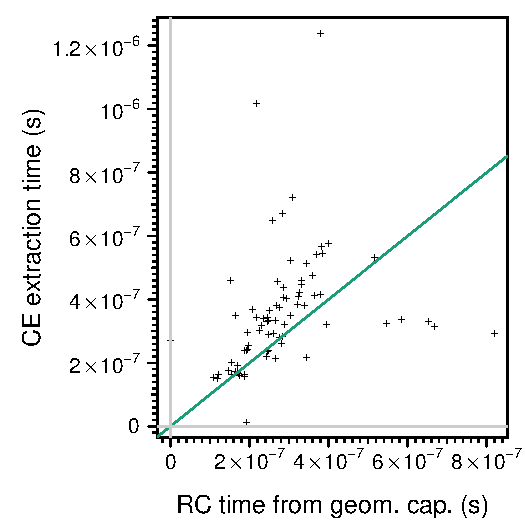
\includegraphics[width=0.45\textwidth]{chargeExtraction_RCtime/CEaBitOfSunExpTime_vs_RCdarkTime.pdf}
			\mycaption[Charge extraction time is related to a RC time.]{Covariance of \acr{ce} extraction time at low light intensity versus the expected time from geometric capacitance (as obtained from dark \acr{dc}). Each point is a different device, many different structures studied during my PhD are represented. The grey line indicates the 1 to 1 relationship.}\label{fig:chargeExtraction_RCtime}
		\end{SCfigure}

		Anyway, during this time, and depending on its location in the device stack, some free charge can recombine.

	\subsubsection{Interpretation of the single measurement}
		From some preliminary and unpublished simulations of \acr{ce} show that a short living exponential decay can be accounted for free charges and a long living and weak exponential decay is caused by a displacement current due to ionic profile updating to the new voltage. The slow decay is not usually measured and seldom reported\cite{ORegan2015b}.

	\subsubsection{Interpretation of the charge versus light bias trend}


\section{Transient PhotoVoltage}\label{interpretation_tpv}

	\subsubsection{Factors Affecting the \acr{tpv}}
		The decays we can observe are limited at long times by the discharge of the extra charge through the oscilloscope resistance and through the device internal resistance, whatever is the smaller. This happens with an RC time of the circuit composed by the capacitance of the device and the \SI{1}{\Mohm} resistance of the oscilloscope or the internal device resistance. The oscilloscope resistance could be varied using an attenuating probe (usually 10X or 100X). This limit to long times is often observed at low light intensities as a plateau in the \acr{tpv} graph. XXXXXXXXXXXXXXXXXXXXXXXXXXXXXXXXXXXXXXXXXXXXXXXXXXXXXXXXXXXXXXXXXXXXXXXXXXXXXXXXX

		\begin{SCfigure}
			\centering
			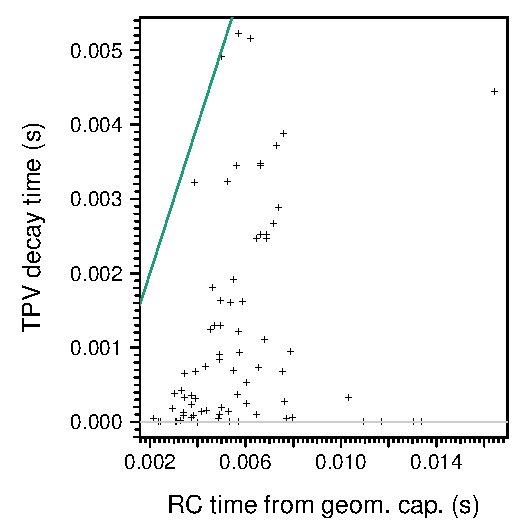
\includegraphics[width=0.45\textwidth]{tpv_RCtime/TPVdarkTime_vs_RCdarkTime.pdf}
			\mycaption[\gls{tpv} time has an upper bond due to discharge through oscilloscope.]{The green line indicates the 1 to 1 relation between the dark \acr{tpv} time (from a robust exponential fit) and the RC time derived from the geometric capacitance from \acr{dc} and the \SI{1}{\Mohm} of the oscilloscope. Each point is a different device.}\label{fig:tpv_RCtime}
		\end{SCfigure}


\section{Transient PhotoCurrent}\label{interpretation_tpc}

\section{Differential Capacitance}\label{interpretation_dc}

	A common commercial capacitor has a capacitance which is a constant, as can be seen in Fig.~\ref{fig:cap_voltage_dependence_commercial}

	\begin{figure}%[!hbtp]%
		\centering
		\begin{subfigure}[t]{0.45\textwidth}
			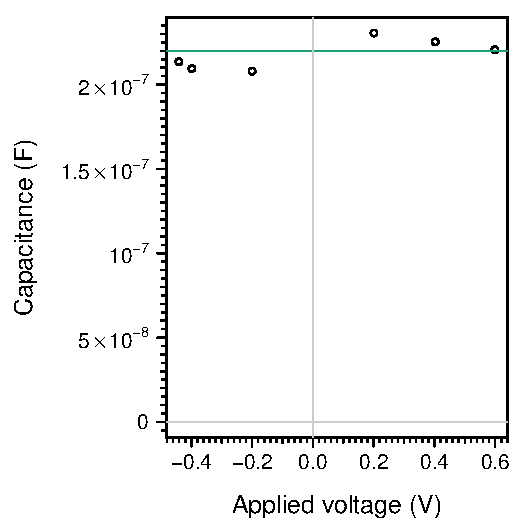
\includegraphics[width=1\textwidth]{cap_voltage_dependence/reference220nF/reference220nF.pdf}
			\subcaption{Commercial \SI{220}{\nano\F} capacitor.}\label{fig:cap_voltage_dependence_commercial}
		\end{subfigure}
		\qquad
		\begin{subfigure}[t]{0.45\textwidth}
			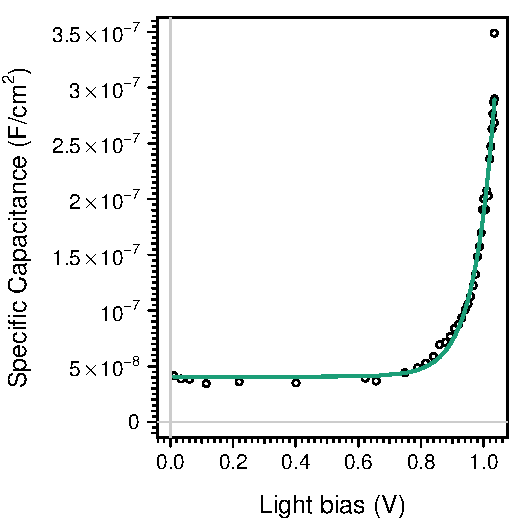
\includegraphics[width=1\textwidth]{cap_voltage_dependence/TAE-1_ig94-1559-1/DC-capacitance-TAE-1_ig94-1559-1.pdf}
			\subcaption{Perovskite solar cell.}\label{fig:cap_voltage_dependence_tae1}
		\end{subfigure}
		\mycaption[Capacitance dependence on applied voltage.]{In (a) the capacitance of a commercial capacitor is reported, it was measured using \acr{ce} with applied voltage bias instead of the classical light bias used for solar cells. The capacitance is obtained as the extracted charge over the applied voltage prior to short circuiting. In (b) the typical capacitance versus voltage profile of a \gls{fto}/\dTiOtwo/\mpTiOtwo/\acr{csfamapbibr}/\tae1/Au device is shown. In this case the indicated voltage is originated by various illumination intensities at open circuit prior to short circuiting.}\label{fig:cap_voltage_dependence}
	\end{figure}
